\section{Cloud application instrumentation}\label{sect:cloud-instrum}

Our solution implements two methods to collect the requirements and
generate the policy. The first is uses ptrace and is based on syscall
argument inspection, the second leverages eBPF, which dynamically
extends the kernel attaching dedicated probes on relevant
\mbox{in-kernel} file system-related events. Both the approaches are
used to instrument the application, however, using ptrace
significantly affects performance and thus is meant to be used only
during staging. On the other hand, eBPF has lighter impact on
performance, hence it can be used also in production.

\subsection{Ptrace-based instrumentation}\label{sect:deep-instr}

Ptrace is a functionality implemented by the kernel aimed at debuggers
and code analysis tools that permits a process, called the {\em
  tracer}, to control and observe the activity performed by another
process, the {\em tracee}. In our implementation, \dmng acts as the
tracer for any application component. To this end, it prepares a
parent and a child process as shown in Figure~\ref{fig:ptrace}, and
then uses the ptrace system call to instruct the kernel that the child
will be traced by the parent (through the PTRACE\textunderscore
  TRACEME request). After this step is completed, \dmng injects into
the child process the component to be run, and then starts it.  While
being traced, every time an event occurs, the tracee is stopped by the
kernel and a notification is sent to the tracer, which has the
possibility to inspect and perform changes before the execution of the
tracee is resumed.  \dmng leverages ptrace to capture all file
system-related syscalls, effectively monitoring the requests issued to
the kernel by the component. The syscalls and their arguments are
recorded by the tracer and saved to the SQLite database mentioned in
Section~\ref{sect:overview}. The set of monitored syscalls includes
interfaces such as open, openat, creat, execve, link, linkat, mkdir,
and the related permission flags (e.g., O\textunderscore APPEND,
O\textunderscore CREAT, O\textunderscore RDONLY). It is
important to point out that \dmng automatically captures and monitors
the possible children spawned by the tracee, and it is also capable to
identify the set of dynamic libraries they depend upon.
% Moreover, when the developer releases the application
% component as a separate library, \dmng also permits to collect the
% dynamic libraries it depends on. To this end it uses {\em ldd}, which
% extracts transient dynamic libraries without running the entire
% application.
% \quest{I've commented this out because it comes out of the blue, and
% without a proper explanation raises more questions than answers}

\begin{figure}[t!]
  \centering
  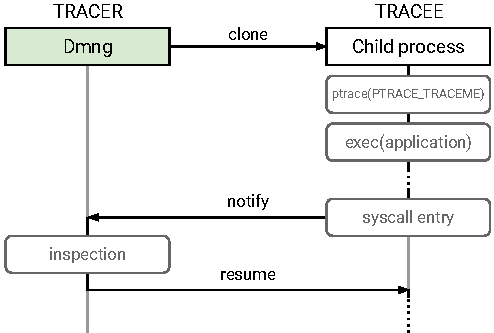
\includegraphics[width=0.6\columnwidth]{chapters/dmng/fig/ptrace_overview.pdf}
  \caption[Architecture of the ptrace-based instrumentation]{\dmng acts as a
    tracer for the application, inspecting the arguments of every
    syscall}
  \label{fig:ptrace}
\end{figure}

When the developer wants to stop the tracing process, \dmng detaches
itself from the tracing of the child process with the
PTRACE\textunderscore DETACH request and it terminates the child
process by sending a SIGKILL signal.

\subsection{eBPF-based intrumentation}\label{sect:cont-monit}

Similarly to other recent security and observability frameworks, like
Cilium~\cite{cilium-repo}, and Tetragon~\cite{tetragon}, \dmng relies
on the eBPF technology to implement continuous monitoring. The eBPF
subsytem allows to change at runtime the behavior of the kernel
without changing its implementation nor adding new modules. Briefly,
it permits to do so by loading compact programs within the kernel,
which are evaluated (without preemption) by a virtual machine-like
component every time a certain hook point is reached. There are many
types of hook within the kernel, examples are network events,
tracepoints, and LSM functions. To store data persistently between
different eBPF program invocations and to share data between kernel
and user space, data structures called {\em maps} are used. They
provide abstractions such as arrays and hashmaps. It is important to
mention that eBPF programs must be safe to run within the kernel and
must not introduce bugs. To ensure these conditions are met, the eBPF
susbsystem automatically performs the two stages of Program
Verification and Just-In-Time Compilation at load time; only if both
terminate without exceptions then the loading of the program is successful.

\begin{figure}[t!]
  \centering
  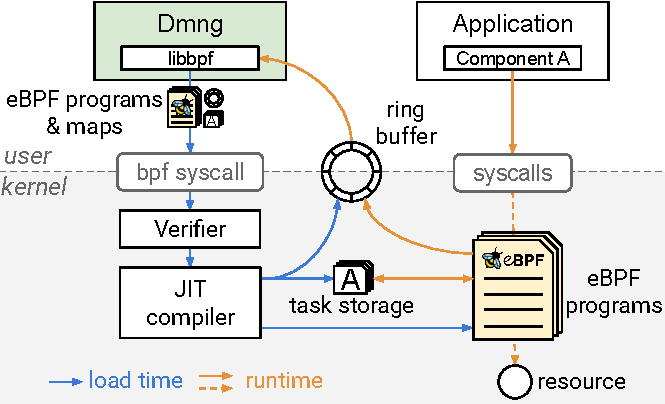
\includegraphics[width=0.7\columnwidth]{chapters/dmng/fig/ebpf_overview.pdf}
  \caption[Architecture of the eBPF-based instrumentation]{\dmng uses
    libbpf to load the eBPF tracing programs and maps, then it polls
    data from the shared ring buffer}
  \label{fig:ebpf}
\end{figure}

\dmng activates eBPF-based tracing on a given application component
using its thread identifier. To this end, it leverages the {\em
  libbpf}~\cite{libbpf-doc} frontend to load into the kernel the eBPF
programs and maps needed to perform tracing, and then starts
collecting data. The process is shown in Figure~\ref{fig:ebpf}.  The
set of eBPF programs comprises of: 1)~dedicated programs to trace the
application component lifetime, and 2)~programs to monitor the file
system-related events generated by the component. The former group of
programs ensure that monitoring extends to tasks spawned through the
clone system call by the component. Hence, they are attached to the
{\em sched\textunderscore process\textunderscore fork} and {\em
  sched\textunderscore process\textunderscore exit} kernel
tracepoints. Instead, the programs that record file system-related
events are attached to hooks reported in
Table~\ref{table-fs-hooks}. Whenever one of these hooks is triggered,
the attached program writes the requirement path and the related
permission to a ring buffer shared with the \dmng user space
process. This permits \dmng to poll data regularly, and then to save it
in the already mentioned SQLite database
(Section~\ref{sect:overview}).

We highlight that the collection of data using this method has minimal
invasiveness: no changes must be introduced in the code of the
application, nor it is necessary to restart it to setup the process.
Indeed, when the developer wants to stop tracing, the eBPF programs
and maps loaded by \dmng are automatically removed, leaving the system
unmodified.

\begin{table}[t]
  \centering
  \small
  \caption{List of file system traced hook points}
  \label{table-fs-hooks}
  \begin{tabular}{ l }
    \toprule
    \multicolumn{1}{ c }{\bf Hook name}\\
    \midrule
    {\tt fentry/security\textunderscore file\textunderscore fcntl}                        \\
    {\tt fentry/security\textunderscore file\textunderscore ioctl}                        \\
    {\tt fentry/security\textunderscore file\textunderscore lock}                         \\
    {\tt fentry/security\textunderscore file\textunderscore mprotect}                     \\
    {\tt fentry/security\textunderscore file\textunderscore open}                         \\
    {\tt fentry/security\textunderscore file\textunderscore receive}                      \\
    {\tt fentry/security\textunderscore file\textunderscore set\textunderscore owner}     \\
    {\tt fentry/security\textunderscore inode\textunderscore getattr}                     \\         
    {\tt fentry/security\textunderscore path\textunderscore chmod}                        \\
    {\tt fentry/security\textunderscore path\textunderscore chown}                        \\
    {\tt fentry/security\textunderscore path\textunderscore chroot}                       \\
    {\tt fentry/security\textunderscore path\textunderscore link}                         \\            
    {\tt fentry/security\textunderscore path\textunderscore mkdir}                        \\    
    {\tt fentry/security\textunderscore path\textunderscore mknod}                        \\
    {\tt fentry/security\textunderscore path\textunderscore rename}                       \\
    {\tt fentry/security\textunderscore path\textunderscore rmdir}                        \\    
    {\tt fentry/security\textunderscore path\textunderscore symlink}                      \\
    {\tt fentry/security\textunderscore path\textunderscore truncate}                     \\
    {\tt fentry/security\textunderscore path\textunderscore unlink}                       \\
    {\tt lsm/bprm\textunderscore check\textunderscore security}                           \\
    {\tt lsm/mmap\textunderscore file}                                                    \\
    \bottomrule
  \end{tabular}
\end{table}


%%% Local Variables:
%%% mode: latex
%%% TeX-master: "../main"
%%% End:
